\documentclass[a0,landscape]{article}
\usepackage{lmodern}
\usepackage{amssymb,amsmath}
\usepackage[margin=0.5in]{geometry}
\usepackage{ifxetex,ifluatex}
\usepackage{fixltx2e} % provides \textsubscript
\ifnum 0\ifxetex 1\fi\ifluatex 1\fi=0 % if pdftex
  \usepackage[T1]{fontenc}
  \usepackage[utf8]{inputenc}
\else % if luatex or xelatex
  \ifxetex
    \usepackage{mathspec}
  \else
    \usepackage{fontspec}
  \fi
  \defaultfontfeatures{Ligatures=TeX,Scale=MatchLowercase}
\fi
% use upquote if available, for straight quotes in verbatim environments
\IfFileExists{upquote.sty}{\usepackage{upquote}}{}
% use microtype if available
\IfFileExists{microtype.sty}{%
\usepackage[]{microtype}
\UseMicrotypeSet[protrusion]{basicmath} % disable protrusion for tt fonts
}{}
\PassOptionsToPackage{hyphens}{url} % url is loaded by hyperref
\usepackage[unicode=true]{hyperref}
\hypersetup{
            pdfborder={0 0 0},
            breaklinks=true}
\urlstyle{same}  % don't use monospace font for urls
\usepackage{graphicx,grffile}
\makeatletter
\def\maxwidth{\ifdim\Gin@nat@width>\linewidth\linewidth\else\Gin@nat@width\fi}
\def\maxheight{\ifdim\Gin@nat@height>\textheight\textheight\else\Gin@nat@height\fi}
\makeatother
% Scale images if necessary, so that they will not overflow the page
% margins by default, and it is still possible to overwrite the defaults
% using explicit options in \includegraphics[width, height, ...]{}
\setkeys{Gin}{width=\maxwidth,height=\maxheight,keepaspectratio}
\IfFileExists{parskip.sty}{%
\usepackage{parskip}
}{% else
\setlength{\parindent}{0pt}
\setlength{\parskip}{6pt plus 2pt minus 1pt}
}
\setlength{\emergencystretch}{3em}  % prevent overfull lines
\providecommand{\tightlist}{%
  \setlength{\itemsep}{0pt}\setlength{\parskip}{0pt}}
\setcounter{secnumdepth}{0}
% Redefines (sub)paragraphs to behave more like sections
\ifx\paragraph\undefined\else
\let\oldparagraph\paragraph
\renewcommand{\paragraph}[1]{\oldparagraph{#1}\mbox{}}
\fi
\ifx\subparagraph\undefined\else
\let\oldsubparagraph\subparagraph
\renewcommand{\subparagraph}[1]{\oldsubparagraph{#1}\mbox{}}
\fi

% set default figure placement to htbp
\makeatletter
\def\fps@figure{htbp}
\makeatother


\date{}

\usepackage{multicol}
\begin{document}
\begin{multicols}{3}
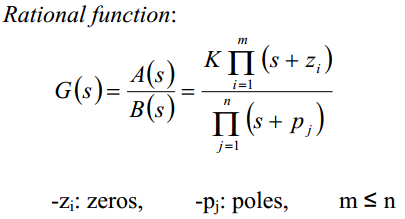
\includegraphics[width=1.77165in,height=0.95669in]{media/image1.png}

\textbf{LAPLACE TRANSFORMS}

Final Value Theorem

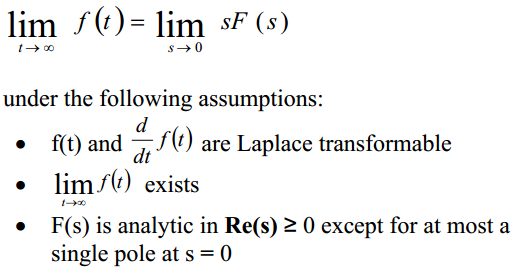
\includegraphics[width=1.77165in,height=0.92126in]{media/image2.png}

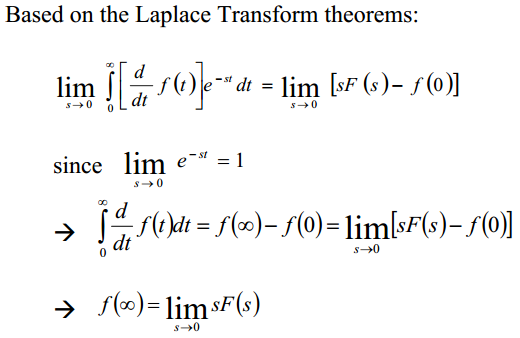
\includegraphics[width=1.77165in,height=1.14961in]{media/image3.png}

Initial Value Theorem

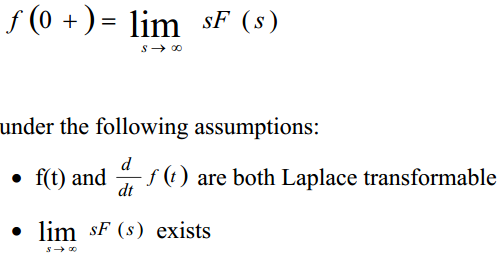
\includegraphics[width=1.77165in,height=0.90551in]{media/image4.png}

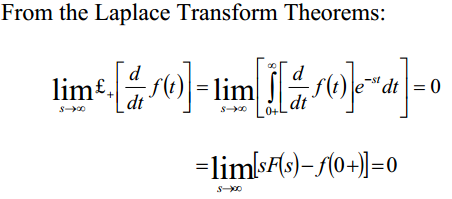
\includegraphics[width=1.77165in,height=0.77953in]{media/image5.png}

\textbf{SOLUTION OF LINEAR DIFFERENTIAL EQUATION}

\[A\ddot{y} + B\dot{y} + Cy = u\left( t \right)\]

\[\text{with\ initial\ conditions\ }\dot{y}\left( 0 \right)\ and\ y(0)\]

\[\text{is\ solved\ by\ constructing\ the\ equation}\]

\[A\left\lbrack s^{2}Y\left( s \right) - sy\left( 0 \right) - \dot{y}\left( 0 \right) \right\rbrack + B\left\lbrack \text{sY}\left( s \right) - y\left( 0 \right) \right\rbrack + CY(s)\]

\[that\ is\ to\ say:\]

\[\mathcal{L}\left\{ \ddot{y} \right\} = s^{2}Y\left( s \right) - sy\left( 0 \right) - \dot{y}(0)\]

\[\text{and}\]

\[\mathcal{L}\left\{ \dot{y} \right\} = sY\left( s \right) - y\left( 0 \right)\]

\textbf{CLOSED LOOP}

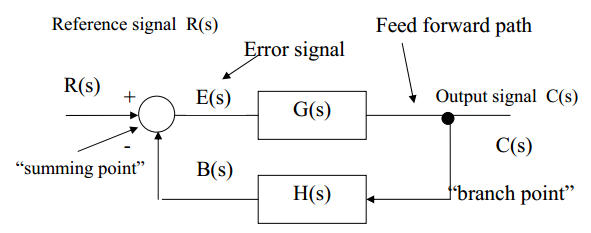
\includegraphics[width=2.56442in,height=1.01101in]{media/image6.png}

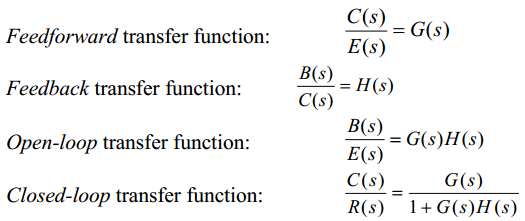
\includegraphics[width=2.55828in,height=1.07691in]{media/image7.png}

\textbf{STATESPACE REPRESENTATIONS}

To generate from a differential equation:

Use the \textbf{closed loop transfer function}

\[\frac{Y\left( s \right)}{U\left( s \right)} = \frac{s + A}{s^{3} + \text{Bs}^{2} + s + A}\]

Separate and take the inverse Laplace transform

\[s^{3}Y\left( s \right) + \text{Bs}^{2}Y\left( s \right) + sY\left( s \right) + AY\left( s \right) = sU\left( s \right) + AU\left( s \right)\]

\[= \dddot{y} + B\ddot{y} + \dot{y} + Ay = \dot{u} + Au\]

Then define state variables:

\(x_{1} = y\) \(\dot{x_{1}} = \dot{y} = x_{2}\)

\(x_{2} = \dot{y}\) \(\dot{x_{2}} = \ddot{y} = x_{3}\)

\(x_{3} = \ddot{y}\)
\(\dot{x_{3}} = \dddot{y} = \dot{u} + Au - B\ddot{y} - \dot{y} - Ay\)

Then construct the state space matrix

\[\begin{bmatrix}
\dot{x_{1}} \\
\dot{x_{2}} \\
\dot{x_{3}} \\
\end{bmatrix} = \begin{bmatrix}
0 & 1 & 0 \\
0 & 0 & 1 \\
 - A & - 1 & - B \\
\end{bmatrix}\begin{bmatrix}
x_{1} \\
x_{2} \\
x_{3} \\
\end{bmatrix} + \begin{bmatrix}
\beta_{1} \\
\beta_{2} \\
\beta_{3} \\
\end{bmatrix}u\]

and

\[y = \begin{bmatrix}
1 & 0 & 0 \\
\end{bmatrix}\begin{bmatrix}
x_{1} \\
x_{2} \\
x_{3} \\
\end{bmatrix} + \beta_{0}u\]

\(\beta\) values can be calculated as follows:

\[\beta_{0} = b_{0}\]

\[\beta_{1} = b_{1} - a_{1}\beta_{0}\]

\[\beta_{2} = b_{2} - a_{1}\beta_{1} - a_{2}\beta_{0}\]

\[\beta_{3} = b_{3} - a_{1}\beta_{2} - a_{2}\beta_{1} - a_{3}\beta_{0}\]

Where the values for \(a_{x}\text{\ and\ }b_{x}\)come from:

\[\dddot{y} + a_{1}\ddot{y} + a_{2}\dot{y} + a_{3}y = b_{0}\dddot{u} + b_{1}\ddot{u} + b_{2}\dot{u} + b_{3}u\]

To perform inverse (find transfer function from statespace model)

\[G\left( s \right) = d + c{(sI - A)}^{- 1}b\]

Where

\[\begin{bmatrix}
\dot{x_{1}} \\
\dot{x_{2}} \\
\dot{x_{3}} \\
\end{bmatrix} = \begin{bmatrix}
A_{11} & A_{12} & A_{13} \\
A_{21} & A_{22} & A_{23} \\
A_{31} & A_{32} & A_{33} \\
\end{bmatrix}\begin{bmatrix}
x_{1} \\
x_{2} \\
x_{3} \\
\end{bmatrix} + \begin{bmatrix}
b_{1} \\
b_{2} \\
b_{3} \\
\end{bmatrix}u\]

And

\[y = \begin{bmatrix}
c_{1} & c_{2} & c_{3} \\
\end{bmatrix}\begin{bmatrix}
x_{1} \\
x_{2} \\
x_{3} \\
\end{bmatrix} + \lbrack d\rbrack u\]

The inverse of a square 2x2 matrix is found by:

\[\begin{bmatrix}
a & b \\
c & d \\
\end{bmatrix}^{- 1} = \frac{1}{ad - bc}\begin{bmatrix}
d & - b \\
 - c & a \\
\end{bmatrix}\]

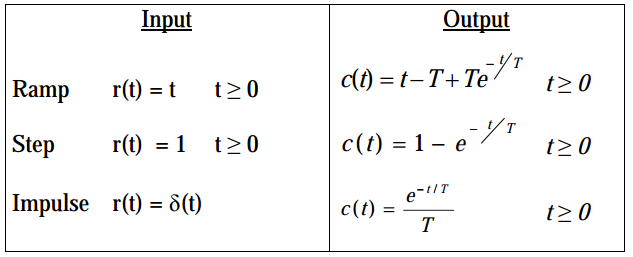
\includegraphics[width=2.52147in,height=1.02367in]{media/image8.png}

\textbf{SECOND ORDER SYSTEMS}

\[G\left( s \right) = \frac{C(s)}{R(s)} = \frac{\omega_{n}^{2}}{s^{2} + 2\zeta\omega_{n}s + \omega_{n}^{2}}\]

\[K = \omega_{n}^{2};\ \ \ \ T = 2\zeta\omega_{n} = 2\sigma;\ \ \ \ \ \zeta = \frac{T}{2\sqrt{K}};\ \ \ \ \omega_{d} = \omega_{n}\sqrt{1 - \zeta^{2}}\]

\[\zeta = damping\ ratio;\ \ \ \ \omega_{n} = undamped\ natural\ frequency\]

\(\sigma = real\ part\ of\ root;\ \ \ \omega_{d} = damped\ natural\ frequency\)

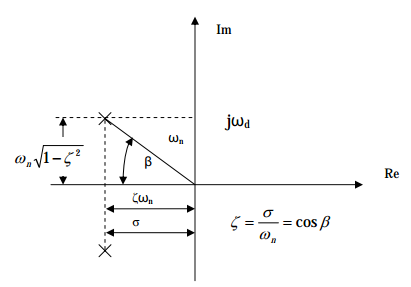
\includegraphics[width=1.96736in,height=1.37361in]{media/image9.png}

\[{Undamped:\ \zeta = 0;\ \backslash n}{Critically\ Damped:\ \zeta = 1;\ \backslash n}{Over\ Damped:\ \zeta > 1}\]

Imaginary axis:

Frequency of oscillations

Real axis:

Decay time

\textbf{UNIT STEP RESPONSE OF A 2\textsuperscript{ND} ORDER UNDAMPED
SYSTEM}

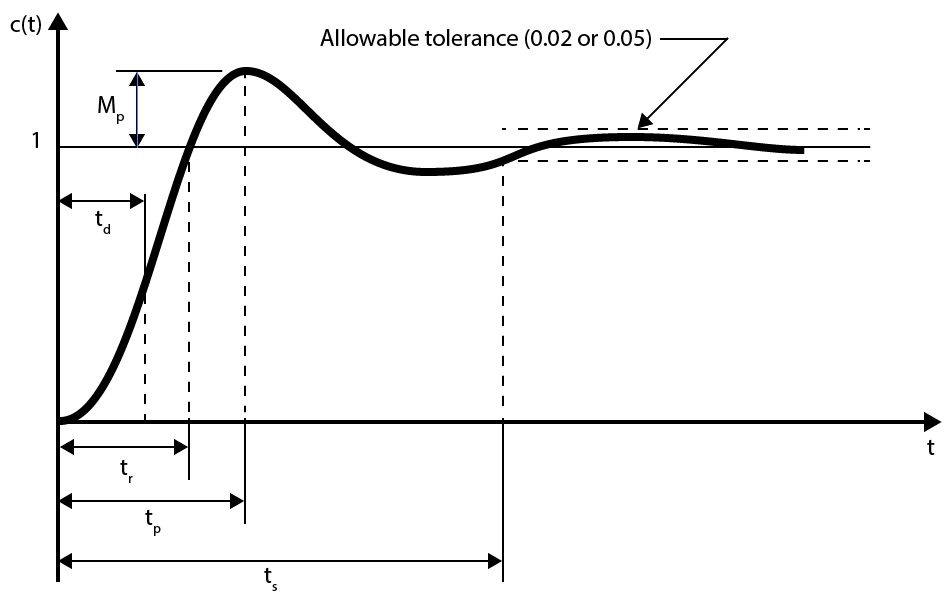
\includegraphics[width=2.83436in,height=1.78813in]{media/image10.png}

\[{t_{d} = delay\ time - to\ reach\ 50\%\ of\ c\left( \infty \right)\text{for\ the\ first\ time}\backslash n}{t_{r} = rise\ time - time\ to\ reach\ 100\%\ of\ c\left( \infty \right)\text{for\ first\ time}\backslash n}{t_{p} = peak\ time - time\ to\ reach\ first\ peak\backslash n}{t_{s} = settling\ time - time\ to\ reach\ \&\ stay\ within\ 2\%\ or\ 5\%\backslash n}{M_{p} = maximum\ overshoot\ \left( \% \right)\backslash n}\]

\[{t_{r} = \frac{1}{\omega_{d}}\operatorname{}\left( - \frac{\omega_{d}}{\sigma} \right);\ \ \ \ t_{p} = \frac{\pi}{\omega_{d}}\backslash n}{M_{p} = e^{- \frac{\zeta\omega_{n}\pi}{\omega_{d}}} = e^{- \frac{\zeta \pi}{\sqrt{1 - \zeta^{2}}}} = e^{- \frac{\sigma \pi}{\omega_{d}}}}\]

\[t_{s} = \frac{4}{\sigma} = \frac{4}{\zeta\omega_{n}}\ \left( 2\%\ band \right);\ \ \ \ t_{s} = \frac{3}{\sigma} = \frac{3}{\zeta\omega_{n}}\ \left( 5\%\ band \right)\]

Dominant poles are the ones closest to the imaginary axis

\textbf{ROUTH-HURWITZ STABILITY TEST}

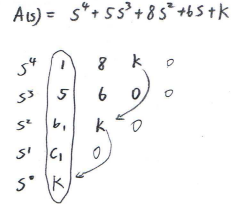
\includegraphics[width=1.48466in,height=1.31009in]{media/image11.png}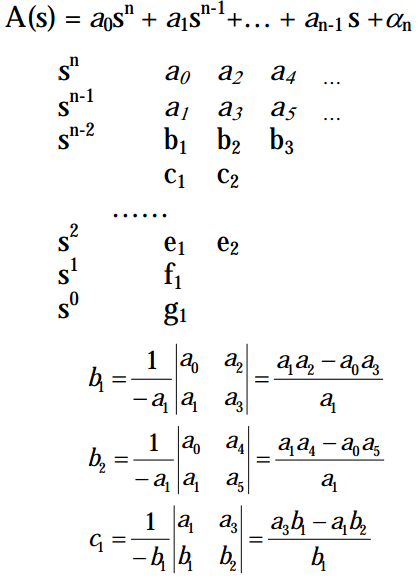
\includegraphics[width=1.91031in,height=2.66258in]{media/image12.png}

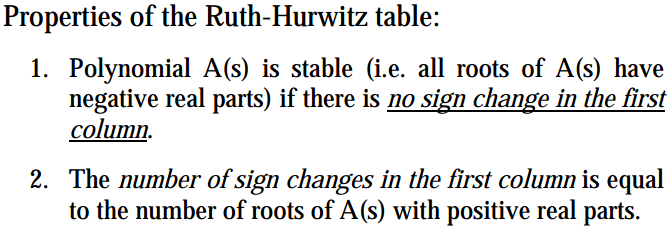
\includegraphics[width=2.44785in,height=0.83792in]{media/image13.png}

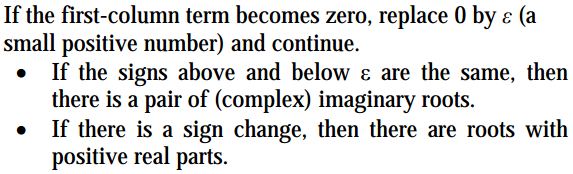
\includegraphics[width=2.39877in,height=0.72842in]{media/image14.png}

\textbf{STEADY STATE ERROR ANALYSIS}

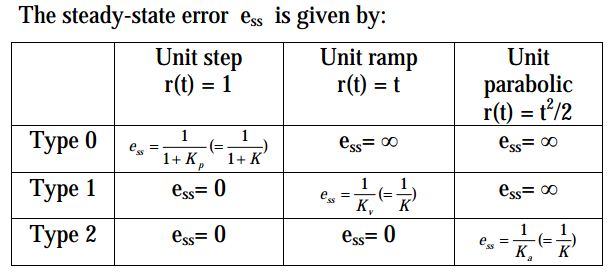
\includegraphics[width=2.94019in,height=1.30675in]{media/image15.png} 
\hfill \break

\[K_{p} = \operatorname{}{G\left( s \right)H(s)}\]

\[K_{v} = \operatorname{}{\text{sG}\left( s \right);\ \ \ \ K_{v} = \operatorname{}{s\left( \text{KG}\left( s \right) \right)}}\]

\[K_{a} = \operatorname{}{s^{2}G\left( s \right);\ \ \ \ K_{a} = \operatorname{}{s^{2}\left( \text{KG}\left( s \right) \right)}}\]

The type of system is determined by the number of poles at the origin.
For example:

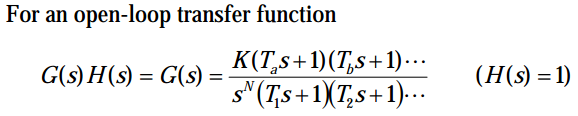
\includegraphics[width=2.60736in,height=0.52328in]{media/image16.png}

\textbf{ROOT LOCUS}

Root Locus presents the poles of the closed loop system when the gain K
changes from zero to infinity.

\textbf{Construction of the Root Locus}

Open loop transfer function

\[\text{KH}\left( s \right)G\left( s \right) = K\frac{B(s)}{A(s)}\]

m: the order of the \textbf{open-loop} numerator polynomial

n: the order of the \textbf{open-loop} denominator polynomial

\textbf{Rule 1:} number of branches equals the number of poles of the
open-loop transfer function

\textbf{Rule 2:} If the total number of poles and zeros of the open-loop
system to the right of the s-point on the real axis is odd, then this
point lies on the locus.

\textbf{Rule 3:} The locus starting point (K=0) are at the open-loop
poles and the locus ending points ($K=\infty$) are at the open loop zeros and
n-m branches terminate at infinity.

\textbf{Rule 4:} Slope of asymptotes of root locus as 's' approaches
infinity

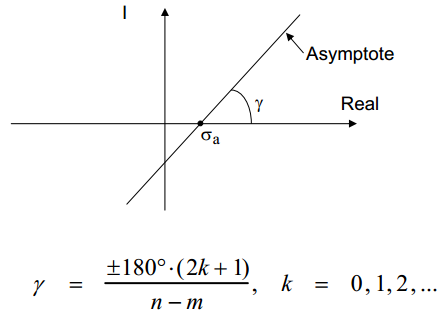
\includegraphics[width=2.27580in,height=1.59509in]{media/image17.png}

\textbf{Rule 5:} Abscissa of the intersection between asymptotes of root
locus and real-axis.

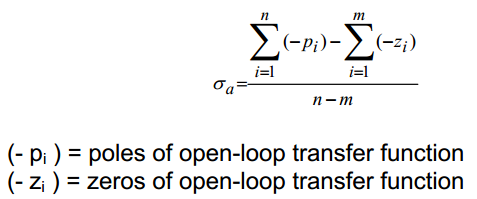
\includegraphics[width=2.13497in,height=0.89069in]{media/image18.png}

\textbf{Rule 6:} Break-away and break-in points. From the characteristic
equation

\[f\left( s \right) = A\left( s \right) + KB\left( s \right) = 0\ \ \ \ and\ \ \ \ K = - \frac{A\left( s \right)}{B\left( s \right)}\]

The break-away and break-in points can be found from

\[\frac{\text{dK}}{\text{ds}} = - \frac{A^{'}\left( s \right)B\left( s \right) - A\left( s \right)B^{'}\left( s \right)}{B^{2}\left( s \right)} = 0\]

\textbf{Rule 7:} Angle of departure from complex poles or zeros.
Subtract from 180° the sum of all angles from all other zeros and poles
of the open-loop system to the complex pole (or zero) with appropriate
signs.

\textbf{Rule 8:} Imaginary-axis crossing points. Use Ruth-Hurwitz table
to find value of K where system becomes unstable.

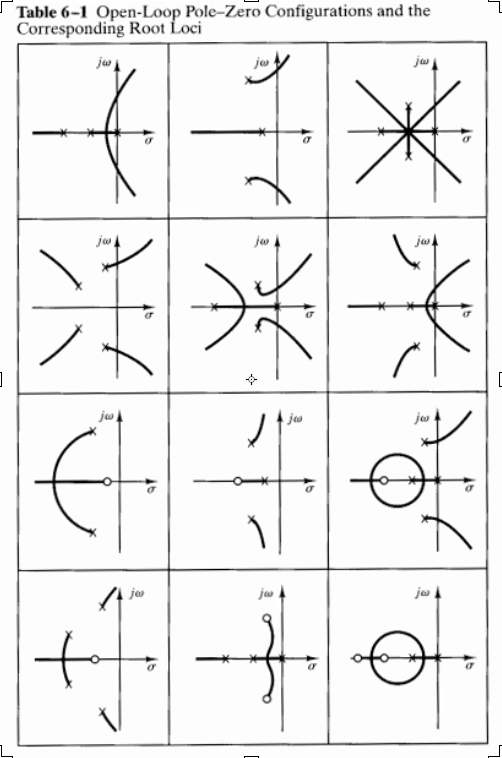
\includegraphics[width=2.22564in,height=3.36063in]{media/image19.png}

\textbf{BODE DIAGRAMS}

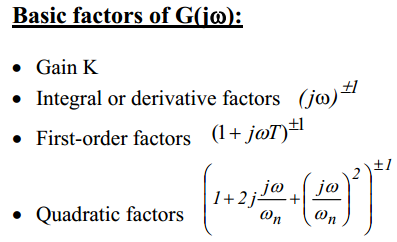
\includegraphics[width=2.08800in,height=1.27279in]{media/image20.png}

\textbf{1. Gain Factor K:} Horizontal straight line at magnitude:
\(20\log{(K)}\text{dB}\)

Phase is zero.

\textbf{2. Integral or derivative factors}
\(\mathbf{(j\omega)}^{\mathbf{\pm 1}}\)

\[\left( \text{j}\omega \right)^{- 1}\  \rightarrow 20\log{\left| \frac{1}{\text{j}\omega} \right| = - 20\log\omega}\]

Magnitude: strait line with slope -20 dB/decade

Phase: -90°

\[\left( \text{j}\omega \right) \rightarrow 20\log\left| \text{j}\omega \right| = 20\log\omega\]

Magnitude: straight line with slope 20dB/decade

Phase: +90°

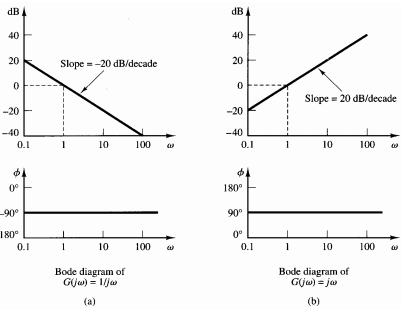
\includegraphics[width=2.24800in,height=1.72199in]{media/image21.png}

\textbf{3. First Order Factors}
\(\left( \mathbf{1 + j\omega T} \right)^{\mathbf{\pm 1}}\)

\[\left( 1 + j\omega T \right)^{- 1} \rightarrow 20\log\left| \frac{1}{1 + j\omega T} \right| = - 20\log\sqrt{1 + \omega^{2}T^{2}}\ \lbrack dB\rbrack\]

Approximation for Magnitude:

\[{\text{For}\ \omega \text{\ between}\ 0\ and\ \frac{1}{T}\  \rightarrow 0 dB\backslash n}{For\ \omega\  \gg \frac{1}{T}\  \rightarrow - 20dB/decade}\]

Phase:

\[{\omega = 0\  \rightarrow \varphi = 0\backslash n}{\omega = \frac{1}{T} \rightarrow \varphi = - 45\backslash n}{\omega = \infty \rightarrow \varphi = - 90}\]

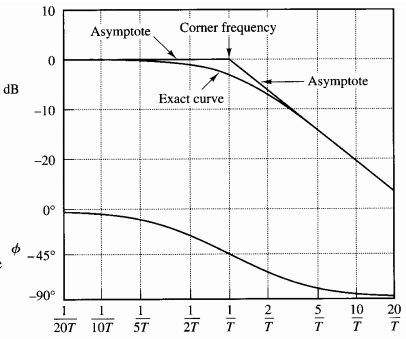
\includegraphics[width=2.55816in,height=2.13600in]{media/image22.png}

\[\left( \mathbf{1 + j\omega T} \right)^{\mathbf{+ 1}}\]

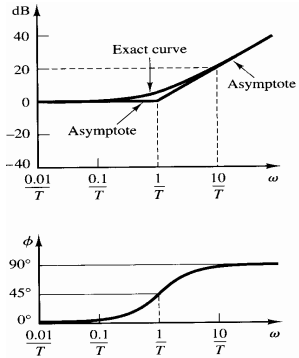
\includegraphics[width=2.05792in,height=2.46400in]{media/image23.png}

\textbf{4. Quadratic Factors}

\[G\left( \text{j}\omega \right) = \frac{1}{1 + 2\zeta\left( \frac{\omega}{\omega_{n}} \right) + \left( \frac{\text{j}\omega}{\omega_{n}} \right)^{2}}\ \ ;\ \ 0 < \zeta < 1\]

Approximation for magnitude:

\[{\omega \ll \omega_{n} \rightarrow 0dB\backslash n}{\omega \gg \omega_{n} \rightarrow - 20\log\left( \frac{\omega^{2}}{\omega_{n}^{2}} \right) = - 40\log{\left( \frac{\omega}{\omega_{n}} \right)\text{dB}}}\]

\[Phase:\]

\[{\omega = 0\  \rightarrow \varphi = 0\backslash n}{\frac{\omega}{\omega_{n}} = 1 \rightarrow \varphi = - 90\backslash n}{\omega = \infty \rightarrow \varphi = - 180}\]

\[{Resonant\ Frequency:\backslash n}{\omega_{r} = \omega_{n}\sqrt{1 - 2\zeta^{2}}\ \ ;\ \ for\ 0 < \zeta < 0.707}\]

\[\backslash n{Resonant\ Peak\ Value:\backslash n}{M_{r} = \left| G\left( \text{j}\omega \right) \right|_{\max} = \frac{1}{2\zeta\sqrt{1 - \zeta^{2}}}\ \ \ ;\ \ for\ 0 < \zeta < 0.707}\]

\[\backslash n\]

Consider

\[G_{1}\left( s \right) = \frac{1}{1 + Ts}\text{\ \ \ \ }G_{2}\left( s \right) = \frac{1}{1 - \text{Ts}}\text{\ \ \ \ }G_{3}\left( s \right) = \frac{1}{\text{Ts} - 1}\text{\ \ \ }\ \]

Then\ldots{}

\[\left| G_{1}(j\omega) \right| = \left| G_{2}(j\omega) \right| = \left| G_{3}(j\omega) \right|\]

And\ldots{}

\[\angle G_{2}\left( \text{j}\omega \right) = - \angle G_{1}\left( \text{j} \omega \right)\text{\ \ \ \ \ \ \ and\ \ \ \ \ \ \ }\angle G_{3}\left( \text{j} \omega \right) = 180 - \angle G_{1}\left( \text{j}\omega \right)\]

\[+ 90\text{\ and\ }\angle G_{3}\left( \text{j}\omega \right)\ goes\ from - 180\ to - 90\]

\[\backslash n\]

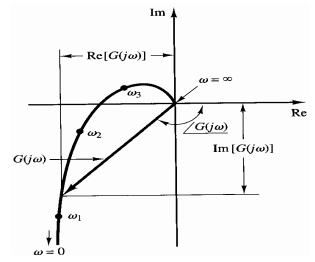
\includegraphics[width=2.10641in,height=1.75200in]{media/image25.png}

Generate based on the Bode Plot.

\textbf{The Nyquist Stability Criterion:} relates the stability of the
closed loop system to the frequency response of the open loop system.

\[Z = N + P\]

\textbf{Z:} Number of zeros of (1+H(S)G(s)) in the right half plane =
number of unstable poles of the closed-loop system.

\textbf{N:} Number of clockwise encirclements of the point -1+j0.

\textbf{P:} Number of poles of G(s)H(s) in the right half plane.

If the plot makes a counter-clockwise encirclement of the -1+j0 point
then N becomes -1.

If Z = 0 the closed loop system is stable. If Z \textgreater{} 0 the
closed loop system has Z unstable poles. If Z \textless{} 0 a mistake
has been made and the calculations need to be rechecked.

\textbf{PHASE AND GAIN MARGINS}

A measure for relative stability of the closed-loop system is how close
\(G(j\omega)\), the frequency response of the open-loop system, comes to
the point -1+j0. This is represented by the phase and gain margins.

\textbf{Phase Margin:} The amount of additional phase lag at the Gain
Crossover Frequency \(\omega_{0}\) required to bring the system to the
verge of instability.

Gain crossover frequency:
\(\omega_{0}\text{\ for\ which\ }\left| G\left( j\omega_{0} \right) \right| = 1\)

Phase margin:
\(\gamma = 180 + \angle G\left( j\omega_{0} \right) = 180 + \phi\)

\textbf{Gain Margin:} The reciprocal of the magnitude
\(\left| G(j\omega_{1}) \right|\) at the Phase crossover frequency
\(\omega_{1}\) required to bring the system to the verge of instability.

Phase crossover frequency:
\(\omega_{1}\ where\ \angle G\left( j\omega_{1} \right) = - 180\)

Gain margin:

\[K_{g} = \frac{1}{\left| G(j\omega_{1}) \right|}\backslash n\]

\[K_{g} = - 20\log\left| G\left( j\omega_{1} \right) \right|\]

\[{K_{g}\ in\ dB > 0 = stable\ \left( \text{for\ minimum\ phase\ systems} \right)\backslash n}{K_{g}in\ dB < 0 = unstable\ \left( \text{for\ minimum\ phase\ systems} \right)}\]

\textbf{Minimum phase systems:} all poles and zeros are in the left half
plane.

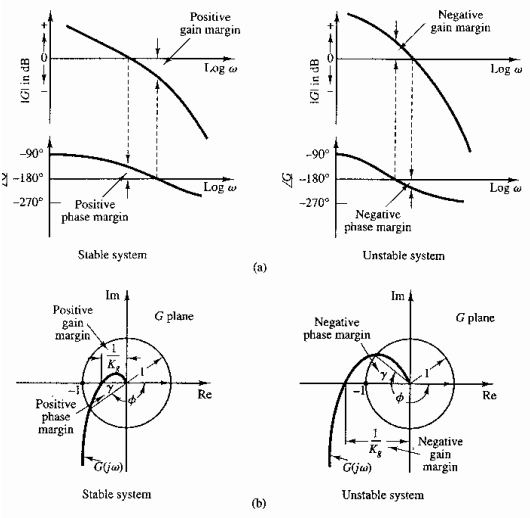
\includegraphics[width=3.35139in,height=3.27551in]{media/image26.png}

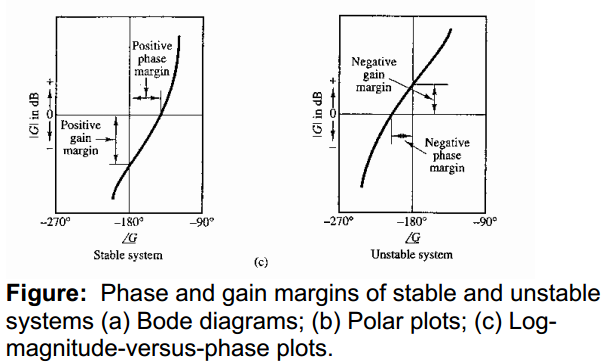
\includegraphics[width=3.35139in,height=1.99763in]{media/image27.png}

If the open-loop system is minimum phase and has both phase and gain
margins positive then the closed-loop system is stable.

For good relative stability both margins are required to be positive.

Good values for minimum phase system are:

Phase Margin: 30°-60°

Gain Margin: above 6dB

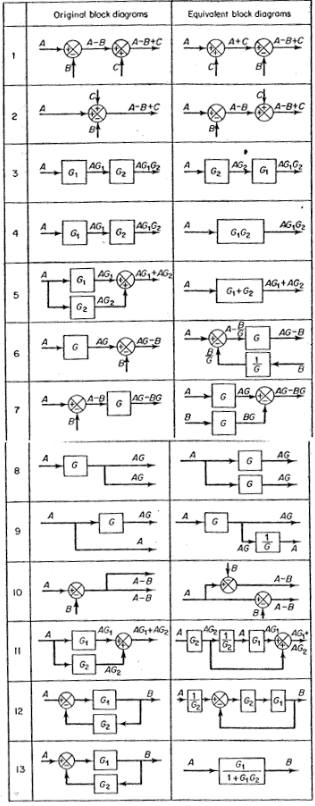
\includegraphics[width=3.03806in,height=7.77358in]{media/image28.png}

\end{multicols}
\end{document}
